\documentclass[11pt,letterpaper]{article}
% --- Packages ---
\usepackage[utf8]{inputenc}
\usepackage[margin=1in]{geometry}
\usepackage{amsmath, amssymb, amsthm, amsfonts}
\usepackage{graphicx}
\usepackage{xcolor}
\usepackage{hyperref}
\usepackage{booktabs}
\usepackage{cite}
\usepackage{microtype}
\usepackage{titlesec}
\usepackage{tcolorbox}
\usepackage{float}
% --- Color Palette (De-saturated, Academic & Professional) ---
\definecolor{ajpblue}{RGB}{28, 54, 115}   % Deep navy accent
\definecolor{ajpsec}{RGB}{54, 95, 145}   % Secondary slate blue
\definecolor{bglight}{RGB}{245, 247, 250} % Light background for callout boxes
\definecolor{bordergrey}{RGB}{210, 215, 223}
% --- Hyperref Setup ---
\hypersetup{
colorlinks=true,
linkcolor=ajpblue,
citecolor=ajpsec,
urlcolor=ajpblue
}
% --- Typography & Headings Styling ---
\titleformat{\section}{\large\bfseries\color{ajpblue}}{\thesection}{1em}{}[{\titlerule[0.5pt]}]
\titleformat{\subsection}{\normalsize\bfseries\color{ajpsec}}{\thesubsection}{1em}{}
% --- Custom Environments for Explanation ---
\newtcolorbox{equationbreakdown}[1]{
colback=bglight,
colframe=ajpblue,
fonttitle=\bfseries,
title={Derivation Details \& Interpretation: #1},
arc=3pt,
boxrule=1pt,
bottomtitle=2mm,
toptitle=2mm
}
\newtcolorbox{physicsinsight}{
colback=bglight,
colframe=ajpsec,
boxrule=0.5pt,
left=4mm,
right=4mm,
top=3mm,
bottom=3mm,
arc=2pt,
sharp corners=false
}
% --- Title & Project Metadata ---
\title{
\vspace{-1.5in}
\rule{\linewidth}{1.5pt} \\ \vspace{4mm}
\large\textbf{PHYSICS GROUP PROJECT REPORT} \\ \vspace{2mm}
\Large\textbf{An Explanatory Guide and Step-by-Step
Derivation of: \\ ``Motion of a Block Slipping on an Arbitrary Surface with Friction''}
\\ \vspace{4mm}
\large\textit{Based on the Article in the American Journal of
Physics} \\
\rule{\linewidth}{1.5pt}
}
% Multi-column author format for a group project
\author{
\begin{tabular}{r @{\quad} l}
\textbf{Project Group:} & [Group 13 / Newton's apple] \\[1ex]
\textbf{Group Members:} & Taehee Hwang
(\textit{Introduction \& Contextual Background,} \\
&
\quad \textit{Mathematical Derivations, Experimental Process)} \\
& Jimin Son (\textit{Abstract, Mathematical Derivations, Experimental Results,} \\
&
\quad \textit{Conclusion}) \\
& Heejin Lee (\textit{Experiment plot, Mathematical Derivations,} \\
&
\quad \textit{Presentation}) \\ [1ex]
\textbf{Course Title:}  & {[General Physics I]} \\
\textbf{Instructor:}    & {Dr. Deniz Olgu Devecioğlu} \\
\textbf{Department:}    & {Department of Physics, DGIST}
\end{tabular}
}
\date{\today}
\begin{document}
\maketitle

\begin{abstract}
This project investigates the theoretical model presented in the American Journal of Physics paper “Motion of a Block Slipping on an Arbitrary Surface with Friction” by Gonzalez-Cataldo, Gutierrez, and Yáñez. The model was applied to a hemispherical acrylic surface to analyze the motion of a sliding rectangular block and determine its departure point. Using video analysis, geometric relationships, projectile motion, and conservation of mechanical energy, the velocities at key locations were calculated and substituted into the analytical equation proposed in the paper to estimate the coefficient of friction. Although the calculated friction coefficient differed significantly from the expected value, the discrepancy revealed the influence of experimental uncertainty and the limitations of the model's idealized assumptions. By reconstructing the intermediate mathematical steps rather than treating the final equation as a black box, this study provides a deeper understanding of how geometry, energy, and friction interact to govern motion on curved surfaces.
\end{abstract}
\tableofcontents
\newpage
% =========================================================================
\section{Introduction \& Contextual Background}
% =========================================================================
The motion of an object sliding on a curved surface is a classical problem in mechanics that combines concepts from dynamics, energy conservation, friction, and differential geometry. A particularly interesting aspect of this problem is determining the point at which the object loses contact with the surface. While this phenomenon is relatively straightforward to analyze for simple geometries such as a sphere or a circular track, it becomes significantly more challenging when the surface has an arbitrary shape and friction is present.

The paper analyzed in this project, \textit{Motion of a Block Slipping on an Arbitrary Surface with Friction} by Gonzalez-Cataldo, Gutierrez, and Yáñez (2017), addresses this general problem. The authors developed a mathematical framework capable of describing the motion of a particle sliding along any concave-downward surface while experiencing friction. Instead of restricting the analysis to a specific geometry, the paper expresses the equations of motion in terms of the local curvature of the surface. This approach allows the velocity of the particle and its departure point to be determined for a wide range of curves, including circles, cycloids, and catenaries. The authors also introduced the concept of a \textit{horizon function}, which provides a geometric criterion for determining when the particle leaves the surface. According to the paper, the departure point is found at the intersection between the particle's dimensionless velocity and the horizon function associated with the curve.

The central physical phenomenon investigated in the paper is the competition between gravitational acceleration, frictional dissipation, and the changing geometry of the surface. As the particle slides downward, gravity tends to increase its speed, while friction reduces its mechanical energy. At the same time, the curvature of the surface determines the normal force required to keep the particle in contact with the track. When the available normal force becomes zero, the particle can no longer follow the surface and departs from it. The paper provides a general mathematical treatment of this departure condition and explores how different surface geometries influence the resulting motion and departure angle.

In this project, the theoretical framework presented in the paper was applied to a hemispherical acrylic surface. Experimental measurements were used to determine the departure point of a sliding rectangular block, estimate its velocity at key locations, and calculate the effective coefficient of friction using the analytical model proposed by the authors. Rather than treating the published equation as a black box, the intermediate mathematical steps were reconstructed and connected to experimentally measurable quantities. This approach made it possible to examine how geometric relationships, projectile motion, energy conservation, and friction combine to determine the motion of the block and its departure from the surfac

% =========================================================================
\section{Step-by-Step Mathematical Derivations}
% =========================================================================
\subsection{Kinematics}
The position of an object in the xy-coordinate system is given as a function of time t by $\mathbf r(t)=(x(t),y(t))$. The velocity and acceleration of the object are defined as $\mathbf v(t)=\frac{d\mathbf r}{dt}$ and $\mathbf a(t)=\frac{d\mathbf v}{dt}$. Under the time interval $[t_0,T]$, where the position vector function r(t) maps to the real plane, the distance traversed by the object is expressed by the following equation.
\begin{equation}
s(t)
=
\int_{t_0}^{t}
\left\|
\frac{d\mathbf r(\tau)}{d\tau}
\right\|
\,d\tau,
\qquad
t\in[t_0,T]
\tag{1}
\end{equation}
At this point, given $\frac{d\mathbf r(t)}{dt}\neq0$ in the interval $[t_0,T]$, the inverse function t(s) exists provided that $\frac{ds(t)}{dt}=\left\|\mathbf r'(t)\right\|=v(t)>0$ and s(t) is an increasing function. Consequently, we can define the function utilizing the Frenet-Serret frame, which is composed of three mutually orthogonal vectors: the tangent vector $\hat{\mathbf t}$ , the principal normal vector $\hat{\mathbf n}$, and the binormal vector $\hat{\mathbf b}$. Each of these vectors is expressed by the following.
\begin{equation}
\hat{\mathbf t}
\equiv
\frac{d\mathbf r}{ds}
\tag{2a}
\end{equation} \begin{equation}
\hat{\mathbf n}
\equiv
\frac{1}{\kappa(s)}
\frac{d\hat{\mathbf t}}{ds}
\tag{2b}
\end{equation} \begin{equation}
\hat{\mathbf b}
\equiv
\hat{\mathbf t}\times\hat{\mathbf n}
\tag{2c}
\end{equation} On the curve s, $\kappa(s)$ denotes the magnitude of curvature, which is given by the following equation. \[
\kappa(s)
=
\left\|
\frac{d\hat{\mathbf t}}{ds}
\right\|
\] If the surface is planar or at an inflection point, κ(s)=0, under which condition the normal vector $\hat{\mathbf n}$ becomes undefined. The binormal vector $\hat{\mathbf b}$ is parallel or antiparallel to the Cartesian unit vector $\hat{\mathbf z}$ ; consequently, taking the dot product of these two vectors results in $\hat{\mathbf b}\cdot\hat{\mathbf z}=\pm1$ This value dictates whether the curve is concave or convex. Accordingly, representing the velocity and acceleration functions through the inverse function t(s) of the curve s(t) yields the following expressions.
\begin{equation}
\mathbf v(t(s))
=
\frac{d\mathbf r}{ds}
\frac{ds}{dt}
=
v(t(s))
\hat{\mathbf t}(s)
\tag{3}
\end{equation}
\begin{equation}
\mathbf a(t(s))
=
\frac{dv(t(s))}{ds}
\frac{ds}{dt}
\hat{\mathbf t}(s)
+
v(t(s))
\frac{d\hat{\mathbf t}(s)}{ds}
\frac{ds}{dt}
\tag{4}
\end{equation}
Since it is known that Eq.(3) and Eq.(4),
\begin{equation}
\mathbf v(s)
=
v(s)\hat{\mathbf t}(s)
\tag{5}
\end{equation}
\begin{equation}
\mathbf a(s)
=
v(s)\frac{dv(s)}{ds}\hat{\mathbf t}(s)
+
v^2(s)\kappa(s)\hat{\mathbf n}(s)
\tag{6}
\end{equation}
We find Eqs.(5) and Eq.(6).
\subsection{Dynamics in the Frenet-Serret frame}
The motion of a particle sliding along a curved surface can be analyzed using the Frenet–Serret coordinate system.
 At this time, according to Newton’s second law, the forces acting on the particle can be expressed as F= ma = W + f + N
, and the tangential equation of motion can be written as \begin{equation}
m v(s)\frac{dv(s)}{ds}
=
m\mathbf g\cdot\hat{\mathbf t}(s)
-\mu N(s)
\tag{7}
\end{equation}
the normal-direction equation of motion is \begin{equation}
m\kappa(s)v^2(s)
=
m\mathbf g\cdot\hat{\mathbf n}(s)
+
(\hat{\mathbf b}\cdot\hat{\mathbf z})N(s)
\tag{8}
\end{equation}
By eliminating N(s), a differential equation for $v^2(s)$ can be obtained.
By multiplying the integrating factor $\exp\!\left(\frac{2\mu}{\hat{\mathbf b}\cdot\hat{\mathbf z}}\int_0^s\kappa(s')\,ds'\right)$ and rearranging,
we obtain \begin{equation}
\frac{d}{ds}
\left[
v^2(s)
e^{\frac{2\mu}{\hat{\mathbf b}\cdot\hat{\mathbf z}}\Phi(s)}
\right]
=
2
e^{\frac{2\mu}{\hat{\mathbf b}\cdot\hat{\mathbf z}}\Phi(s)}
\left[
\mathbf g\cdot\hat{\mathbf t}(s)
+
\mu
\frac{\mathbf g\cdot\hat{\mathbf n}(s)}
{\hat{\mathbf b}\cdot\hat{\mathbf z}}
\right]
\tag{9}
\end{equation}
where \begin{equation}
\Phi(s)
\equiv
\int_0^s \kappa(s')\,ds'
\tag{10}
\end{equation}
Integrating Eq. (9) from 0 to s yields, we can obtain \begin{equation}
v^2(s)
=
v_0^2
e^{-\frac{2\mu}{\hat{\mathbf b}\cdot\hat{\mathbf z}}\Phi(s)}
+
2
e^{-\frac{2\mu}{\hat{\mathbf b}\cdot\hat{\mathbf z}}\Phi(s)}
\int_0^s
\left[
\mathbf g\cdot\hat{\mathbf t}(s')
+
\mu
\frac{\mathbf g\cdot\hat{\mathbf n}(s')}
{\hat{\mathbf b}\cdot\hat{\mathbf z}}
\right]
e^{\frac{2\mu}{\hat{\mathbf b}\cdot\hat{\mathbf z}}\Phi(s')}
\,ds'
\tag{11}
\end{equation}
This is the most general equation representing the velocity of a particle moving on a curved surface. Here, we set $\Phi(0)=0$ and the initial velocity as $v(0)\equiv v_0$. In addition, since the arc length s is always increasing and uniquely defined, it can be used to express the motion of the particle. However, in most cases, it is difficult to analytically calculate the arc length, making it impossible to solve the equation directly. To resolve this issue, the calculation is performed using the tangent angle.
Finding the value of N from Eq. (7), we can obtain \begin{equation}
N(s)
=
mv^2(s)\frac{\kappa(s)}{\hat{\mathbf b}\cdot\hat{\mathbf z}}
-
m\frac{\mathbf g\cdot\hat{\mathbf n}(s)}
{\hat{\mathbf b}\cdot\hat{\mathbf z}}
\tag{12}
\end{equation} When N(s) = 0, (when the object is not in contact with the surface), we obtain the following. \begin{equation}
\frac{v^2(s)}{gR}
=
\frac{1}{gR}
\frac{\mathbf g\cdot\hat{\mathbf n}(s)}
{\kappa(s)}
\tag{13}
\end{equation} At this time, the right side of the equation is defined as\begin{equation}
H(s)
\equiv
\frac{1}{gR}
\frac{\mathbf g\cdot\hat{\mathbf n}(s)}
{\kappa(s)}
\tag{14}
\end{equation} 
For the particle to remain in contact with the surface, the magnitude of the normal force must be greater than zero. On a convex upward curve, $\hat{\mathbf b}\cdot\hat{\mathbf z}=-1$.
So according to Eq. (14), the condition $N(s)\ge0$ is expressed in the following form \begin{equation}
\frac{v^2(s)}{gR}
\le
H(s)
\tag{15}
\end{equation}
Therefore, H represents the velocity criterion that the particle must reach to lose contact with the surface. In particular, when s = 0,\begin{equation}
\left(
\frac{v_0^2}{gR}
\right)^{(\max)}
=
H(0)
=
\frac{\mathbf g\cdot\hat{\mathbf n}(0)}
{gR\,\kappa(0)}
\tag{16}
\end{equation} holds true. If the equality holds in this equation (if the initial velocity reaches the horizon), the particle immediately detaches from the surface and moves along a parabolic trajectory above the surface. Therefore, the maximum initial velocity that can be given to the particle is determined by this condition.

\subsection{Tangent angle}

The vector in the $\hat{t}$ direction has a positive x-component and a negative y-component, which can be expressed as (18). Here $\Phi$ is the angle formed by the tangent line.

 \begin{equation}
    \hat{t}= cos\varphi\hat{x}- sin\varphi\hat{y} 
 \tag{18}
 \end{equation}
By using (18) and (2b), $\hat{n}$ can be rewritten as (19).
\begin{equation}
    \hat{n}\equiv \frac{1}{k(s)} \frac{\mathrm{d} \hat{t}}{\mathrm{d} s} 
    \tag{2b}
\end{equation}
\begin{equation}
\hat{n}=-\frac{(d\varphi/ds)}{k(s)} 
[sin\varphi\hat{x}+cos\varphi\hat{y}]
    \tag{19}
\end{equation}
At this time, since $\hat{n}$ is a unit vector, $\left\vert \hat{n} \right\vert = 1$, which indicates that the magnitude of the absolute value on the right hand side is also 1; thus, it can be derived from Eq.(19) that $k(s)=\left\vert d\varphi / ds \right\vert$. Here, as the angle $\phi$ increases as the object falls, it becomes $d\varphi / ds > 0$, which leads to $k(s)=d\varphi / ds$. This enables the expression as $\int k(s)ds=\varphi(s)$, allowing $\Phi(s) \equiv \int_{0}^{s}k(s')ds' (11)$ to be represented as $\Phi(s) = \varphi(s) - \varphi_0$.
Furthermore, in the coordinate system, the b-axis and the z-axis are parallel to each other but point in opposite directions, so it can be expressed as $\hat{b} \cdot \hat{z}=-1$. Based on the above, (12) yields (20). Moreover, since the gravitational acceleration g acts only in the y-axis direction $g=-g\hat{y}$, we can set $\varphi \equiv \varphi(s), \varphi'\equiv\varphi(s')$. By expressing the velocity as$ v(s(\varphi))\equiv v(\varphi)$, (15) can be represented as (21)
At this time, $H(s(\varphi))\equiv H(\varphi)$ and $k(s(\varphi)=k(\varphi)$. All of the above processes were carried out assuming a scenario on a convex upward curved surface.

\begin{equation}
\begin{split}
    v^2(\varphi) = {}& v_0^2 e^{2\mu(\varphi-\varphi_0)}+2g e^{2\mu\varphi}\\& \times \int_{\varphi_0}^{\varphi}(\sin \varphi' - \mu\cos\varphi') \frac{e^{-2\mu\varphi'}}{\kappa(\varphi')}d\varphi'
\end{split}
\tag{20}
\end{equation}
\begin{equation}
    H{(\varphi)}= \frac{1}{\mathbf g R} \frac{\mathbf{g}\cdot\hat{\mathbf{n}}}{\kappa(\varphi)}=\frac{\cos\varphi}{R\kappa(\varphi)}
    \tag{21}
\end{equation}

\subsection{Departure from the circle}
Expressing the circle through parameterization with respect to $\phi$  yields $r(\varphi) = (Rsin\varphi, Rcos\varphi)$, where $\varphi \in [0, \pi/2]. $

1. Relative to the vertical axis, the magnitude of curvature of a circle with radius R is defined as $k(\phi)=1/R$
As $\phi$ is an increasing variable, Eq.(20) reduces to Eq.(22). Consequently, integration using the exponential forms of $sin\phi$ and $cos\phi$ results in Eq.(23)
\begin{equation}
    \begin{split}
        \frac{v^2(\varphi)}{\mathbf g R}= {} & \frac{v_0^2}{\mathbf g R} e^{2\mu\varphi} \\ & + 2 e^{2\mu\varphi} \int_{0}^{varphi} (\sin \varphi' - \mu\cos\varphi') e^{-2\mu\varphi'} d\varphi'.   
    \end{split}
    \tag{22}
\end{equation}
\begin{equation}
    \begin{split}
        \frac{v^2(\varphi)}{\mathbf g R}= {}& \frac{v_0^2}{\mathbf g R}e^{2\mu\varphi} \\ & + \frac{(2-4\mu^2)(e^{2\,u\varphi}-\cos\varphi)-6\mu\sin\varphi}{1+4\mu^2}
    \end{split}
    \tag{23}
\end{equation}

2. Relative to the horizontal axis, the horizontal line corresponding to Eq. (21) within the circle reduces to $H(\varphi)=\cos\varphi$

This indicates that prior to leaving the surface, the velocity of the object must satisfy Eq.(24).
\begin{equation}
    \frac{v^2(\varphi)}{\mathbf g R} \le \cos\varphi
    \tag{24}
\end{equation}

According to Eq.(17), the maximum initial velocity of the object is given by Eq.25
\begin{equation}
    \left(\frac{v_0^2}{\mathbf g R} \right)^{(\text{max})}=1\
    \tag{25}
\end{equation}

In the case where $\mu=0$, Eq.26
\begin{equation}
    v^2(\varphi)=v_0^2 + 2\mathbf g R(1-\cos\varphi)
    \tag{26}
\end{equation}

The particle detaches from the surface when Eq.27
\begin{equation}
    \cos\varphi - \frac{2}{3}+\frac{v_0^2}{3\mathbf g R}
\tag{27}
\end{equation}

\subsection{Coefficient of kinetic friction between acrylic plate and wood}
Among the sources with clear referenves, the friction coefficient between acrylic and steel, which ranges from 0.4 to 0.5 represents the material interface most similar to our experimental setup
(https://us.misumi-ec.com/blog/coefficient-of-friction/)

% =========================================================================
\section{Experimental Process}
% =========================================================================

\subsection{Materials List }
Rectangular parallelepiped blocks , Transparent hemisphere (21 cm in diameter) , Digital camera , Inclined plane (constructed from an L-shaped plastic folder),  Measuring tape
\subsection{Experimental Procedure}
\begin{enumerate}
    \item The initial drop height of the object is measured.

    \item The inclined plane is secured to the apex of the transparent hemisphere.

    \item A camera is positioned perpendicularly to the ground to record the experiment.

    \item The block is released from the inclined plane to slide downward.

    \item The initial velocity at the apex of the hemisphere is calculated using the law of conservation of mechanical energy.

    \item The detachment angle, at which the block separates from the surface of the hemisphere, is measured through video analysis.

    \item The velocity at the exact moment of detachment is determined using the position and time coordinates of the block at an arbitrary point after separation.

    \item The friction coefficient of the acrylic hemisphere is calculated by substituting the obtained values into the governing equations from previous literature.

    \item The experimental error is determined by comparing the measured friction coefficient of the acrylic hemisphere with its theoretical value.

    \item The potential sources of experimental error are analyzed and discussed.
\end{enumerate}

\section{Experimental Results}

\subsection{Measurements in a Stationary State}

\begin{itemize}
    \item Gravitational acceleration: $g = 9.8\,\mathrm{m/s^2}$
    \item Mass of the rectangular block: $m = 0.0173\,\mathrm{kg}$
    \item Radius of the hemisphere: $R = 0.1010\,\mathrm{m}$
    \item Initial height: $h_0 = 0.2880\,\mathrm{m}$
\end{itemize}

\subsection{Measurement at Departure Point A}

\begin{figure}[H]
    \centering
    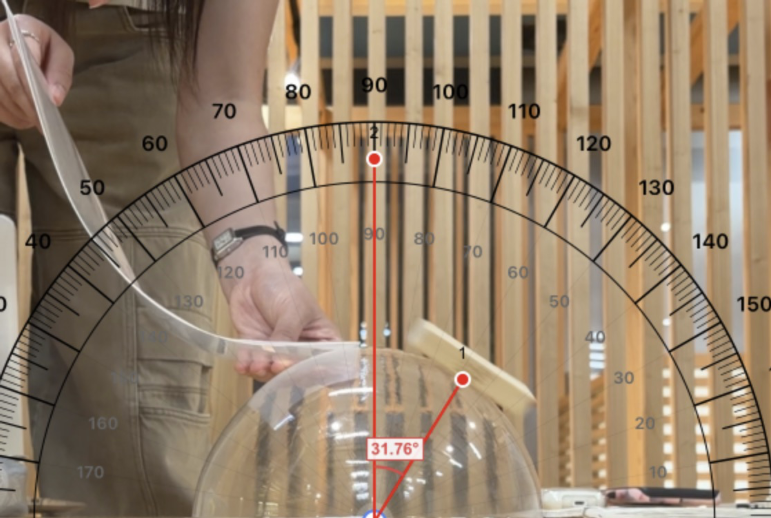
\includegraphics[width=0.5\linewidth]{KakaoTalk_20260613_000212322.png}
    \caption{Determination of departure point A}
    \label{fig:placeholder}
\end{figure}

The point at which the rectangular block leaves the hemispherical surface is defined as Point A. The angle measured from the central axis of the hemisphere was determined using a digital protractor application. The measured angle was $31.76^\circ$, which corresponds to $\theta = 0.5543165704\,\mathrm{rad}$.

\begin{figure}[H]
    \centering
    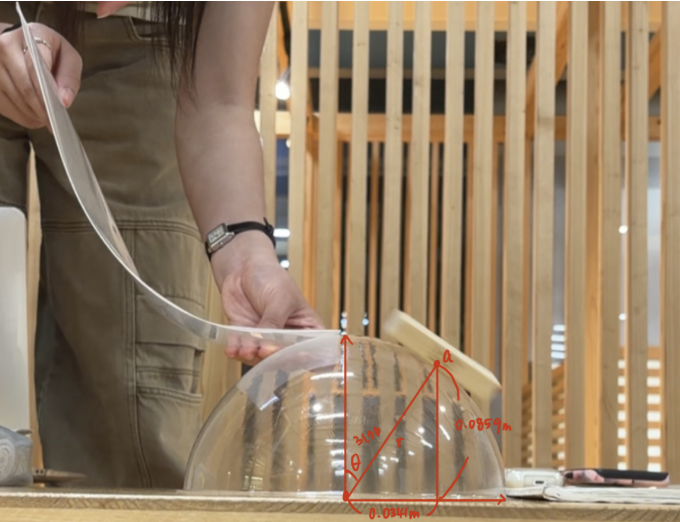
\includegraphics[width=0.5\linewidth]{KakaoTalk_20260613_004007596.png}
    \caption{Geometric measurements at Point A}
    \label{fig:placeholder}
\end{figure}


Using the radius of the hemisphere and the measured angle, the height of Point A and the horizontal distance between Point A and the central axis were calculated. The height was found to be $0.08588\,\mathrm{m}$ and the horizontal distance was $0.05316\,\mathrm{m}$.

By analyzing the video frames, the time required for the block to travel from the top of the hemisphere to Point A was determined to be $0.42\,\mathrm{s}$.

\begin{table}[h]
\centering
\caption{Measurements at Point A}
\begin{tabular}{lc}
\hline
Parameter & Value \\
\hline
$\theta$ & $0.5543165704\,\mathrm{rad}$ \\
Height at Point A & $0.08588\,\mathrm{m}$ \\
Distance from Point A to the central axis & $0.05316\,\mathrm{m}$ \\
Time to reach Point A & $0.42\,\mathrm{s}$ \\
\hline
\end{tabular}
\end{table}

\subsection{Measurement of Point B}

\begin{figure}[H]
    \centering
    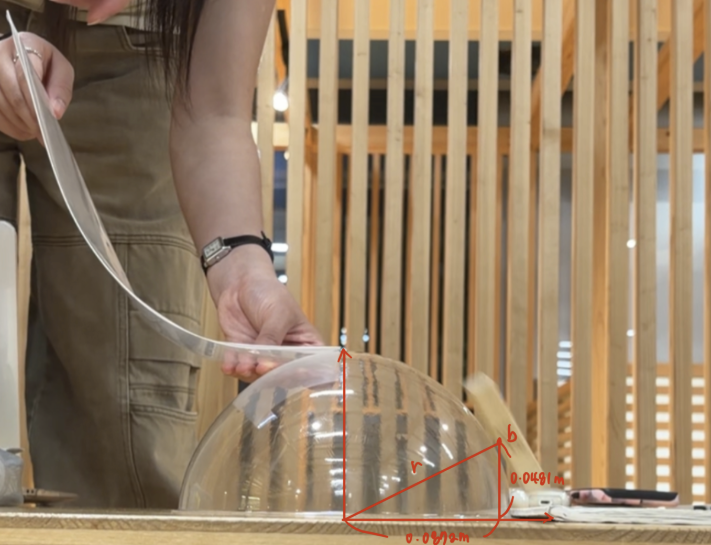
\includegraphics[width=0.5\linewidth]{KakaoTalk_20260613_004033328.png}
    \caption{Enter Caption}
    \label{fig:placeholder}
\end{figure}

To determine the velocity at Point A, an arbitrary point after departure was selected and defined as Point B. The time required for the block to travel from the top of the hemisphere to Point B was measured to be $0.47\,\mathrm{s}$.

Using the pixel dimensions in the image and the known dimensions obtained at Point A, proportional calculations were performed. The height of Point B was found to be $0.0481\,\mathrm{m}$, and the horizontal distance from Point B to the central axis was $0.08722\,\mathrm{m}$.

\begin{table}[h]
\centering
\caption{Measurements at Point B}
\begin{tabular}{lc}
\hline
Parameter & Value \\
\hline
Height at Point B & $0.0481\,\mathrm{m}$ \\
Distance from Point B to the central axis & $0.08722\,\mathrm{m}$ \\
Time to reach Point B & $0.47\,\mathrm{s}$ \\
\hline
\end{tabular}
\end{table}

\subsection{Determination of the Velocity at the Top of the Hemisphere}

First, the initial gravitational potential energy is calculated:

\[E_{p,0}=mgh
=(0.0173)(9.8)(0.288)
=0.04882752\,\mathrm{J}\]

Therefore, the initial potential energy is

\[E_{p,0}=0.04882752\,\mathrm{J}.\]

Next, the gravitational potential energy at the top of the hemisphere is

\[E_{p,t}=mgh
=(0.0173)(9.8)(0.101)
=0.01712354\,\mathrm{J}.\]

Therefore,

\[
E_{p,t}=0.01712354\,\mathrm{J}.
\]

Assuming conservation of mechanical energy, the kinetic energy at the top of the hemisphere is

\[
E_k
=E_{p,0}-E_{p,t}
=0.04882752-0.01712354
=0.03170398\,\mathrm{J}.
\]

Since kinetic energy is given by

\[
E_k=\frac{1}{2}mv^2,
\]

the velocity at the top of the hemisphere is

\[
v
=
\sqrt{\frac{2E_k}{m}}
=
\sqrt{\frac{2(0.03170398)}{0.0173}}
=
1.914471206\,\mathrm{m/s}.
\]

\subsection{Determination of the Velocity at Point A}

The travel time from Point A to Point B was

\[
t=0.47-0.42=0.05\,\mathrm{s}.
\]

The horizontal displacement between Points A and B was

\[
\Delta x
=
0.08722-0.05316
=
0.03406\,\mathrm{m}.
\]

The vertical displacement was

\[
\Delta y
=
0.08588-0.04810
=
0.03778\,\mathrm{m}.
\]

Let the horizontal and vertical velocity components at Point A be $v_x$ and $v_y$, respectively.

From horizontal motion,

\[
v_xt=\Delta x
\]

\[
v_x
=
\frac{0.03406}{0.05}
=
0.6812\,\mathrm{m/s}.
\]

From vertical motion,

\[
\frac{1}{2}gt^2+v_yt
=
0.03778,
\]

\[
\frac{1}{2}(9.8)(0.05)^2
+
0.05v_y
=
0.03778,
\]

\[
v_y
=
0.5106\,\mathrm{m/s}.
\]

The speed at Point A is therefore

\[
v
=
\sqrt{v_x^2+v_y^2}
=
\sqrt{(0.6812)^2+(0.5106)^2}
=
0.8513200338\,\mathrm{m/s}.
\]

\subsection{Determination of the Coefficient of Friction of the Acrylic Surface}

Substituting the measured values into equation (23) provided in the referenced literature,

\[
v = 0.8513200338\,\mathrm{m/s},
\]

\[
v_0 = 1.914471206\,\mathrm{m/s},
\]

\[
\theta = 0.5543165704\,\mathrm{rad},
\]

\[
R = 0.101\,\mathrm{m},
\]

\[
g = 9.8\,\mathrm{m/s^2},
\]

the coefficient of friction is obtained as

\[
\mu = -1.17.
\]

The experimentally calculated value differs significantly from the known coefficient of friction of acrylic, which is approximately

\[
\mu \approx 0.45.
\]

This discrepancy indicates that considerable experimental error exists in the measurements or assumptions used in the analysis.
```


% =========================================================================
\section{Conclusion}
% =========================================================================

This project successfully reproduced and examined the motion of a block sliding on a hemispherical surface by applying the mathematical framework presented in the original American Journal of Physics paper. Rather than relying solely on the final equation provided in the literature, the intermediate mathematical operations were unpacked and connected to measurable physical quantities such as position, velocity, energy, and the coefficient of friction. This process clarified how the theoretical model links the geometry of the surface to the dynamics of the moving object and provided a deeper understanding of the physical mechanisms governing detachment from the hemisphere.

The experimentally obtained negative friction coefficient indicates a fundamental mismatch between the assumptions of the idealized model and the conditions of the actual experiment. The primary source of discrepancy originated from the estimation of the initial velocity at the top of the hemisphere. The calculation assumed perfect conservation of mechanical energy along the guiding track and neglected frictional losses before the block reached the hemispherical surface. As a result, the theoretical apex velocity was significantly overestimated.

Additional uncertainty arose in the determination of the velocity at the detachment point. Air resistance acting on the block after separation reduced its actual speed, while the pixel-based motion analysis introduced further measurement errors due to image resolution limits, motion blur, and perspective effects. These factors collectively contributed to an underestimation of the post-detachment velocity.

Because the theoretical model predicted an initial velocity that was larger than the experimentally inferred detachment velocity, the governing equation compensated for this inconsistency by producing a non-physical negative friction coefficient. Although the calculated value did not match the known friction coefficient of acrylic, the discrepancy itself provided valuable insight into the sensitivity of the model to experimental uncertainties and simplifying assumptions.

Overall, this project demonstrated how theoretical equations derived in the literature can be tested using real experimental data and highlighted the importance of carefully examining each mathematical step. By unpacking the intermediate calculations rather than treating the published equation as a black box, it became possible to identify the physical meaning of each term, evaluate the validity of the underlying assumptions, and better understand the relationship between mathematical models and real-world motion.

% =========================================================================
\begin{thebibliography}{99}
% =========================================================================
\bibitem{originalpaper}
Felipe Gonzalez-Cataldo, Gonzalo Gutierrez, \& Julio M. Ya~ nez. (2017).
``Sliding down an arbitrary curve in the presence of friction.''
\textit{American Journal of Physics}, 85(2), 108--114.

\end{thebibliography}

Github Link: https://github.com/hsjimin35-coder/General-Physics-Group-13-Newton-s-Apple


\end{document}